\documentclass[aspectratio=169]{beamer}
\usepackage{siunitx,booktabs,xcolor,xspace,multirow,graphicx,lipsum}
\usepackage[spanish,mexico,es-noindentfirst]{babel}
\usepackage[utf8]{inputenc}
\usepackage{tikz}
\usetikzlibrary{shapes,arrows.meta,positioning,calc,fit,backgrounds,shadows,decorations.pathreplacing}
\usepackage{subcaption}
\usepackage[charter]{mathdesign}
\usetheme{Madrid}
\usepackage{tcolorbox}
\usepackage{hyperref}

\usefonttheme{serif}


\setbeamertemplate{frametitle}{
  \begin{beamercolorbox}[wd=\paperwidth,ht=1cm, sep=0.25cm]{frametitle}
    \begin{tikzpicture}[remember picture,overlay]
      \node[anchor=north east] at (current page.north east) {
\includegraphics[height=0.75cm]{figuras/inetSys-fundo-azul-logo.png}};
    \end{tikzpicture}
    \usebeamerfont{frametitle}\bfseries\insertframetitle
  \end{beamercolorbox}
}

\setbeamertemplate{caption}[numbered]
\setbeamercolor{frametitle}{bg=beamer_color,fg=white}
\setbeamercolor{author in head/foot}{bg=beamer_color,fg=white}
\setbeamercolor{title in head/foot}{bg=beamer_color,fg=white}
\setbeamercolor{date in head/foot}{bg=beamer_color,fg=white}
\setbeamercolor{titlelike}{parent=structure,bg=beamer_color,fg=white}
\setbeamertemplate{section in toc}[sections numbered]
\setbeamertemplate{subsection in toc}[subsections numbered]
\setbeamerfont{section in toc}{series=\bfseries}
\setbeamercolor{section in toc}{fg=black}
\setbeamercolor{caption name}{fg=blue}
\setbeamerfont{caption name}{series=\bfseries}
\setbeamerfont{caption}{size=\small}
\setbeamercolor{bibliography entry author}{fg=black}
\setbeamercolor{bibliography entry title}{fg=black} 
\setbeamertemplate{section in toc}{\inserttocsectionnumber.~\inserttocsection\par}
\setbeamertemplate{subsection in toc}{\hspace{1.5em}\inserttocsectionnumber.\inserttocsubsectionnumber~\inserttocsubsection\par}



\title[\textbf{}]{\textbf{SAC-FTOPSIS: Um Modelo de Decisão para o Descarregamento de Tarefas em Redes Veiculares}}
\author[\textbf{Antônio Sérgio de Sousa Vieira}]{\textbf{Antônio Sérgio de Sousa Vieira \break sergio.vieira@ifce.edu.br}}
\date{}

\renewcommand{\maketitle}{
\begin{center}
    
\includegraphics[height=0.8cm]{figuras/ifce.pdf}\hspace{0.5cm}
    
\includegraphics[height=0.8cm]{figuras/uece_inetsys_desc_logo.png}
    \\[0.1cm]
    \textbf{\scriptsize DOUTORADO EM CIÊNCIA DA COMPUTAÇÃO}
\end{center}

\vspace{-1.8\baselineskip}
\titlepage
\vspace{-3.2\baselineskip}

\begin{center}
    \tiny
    \begin{tabular}{rl}
        \textbf{Orientador:} & Dr. Joaquim Celestino Júnior (UECE) \\
        \textbf{Coorientador:} & Prof. Dr. Alisson Barbosa de Souza (UFC) \\
    \end{tabular}

    \vspace{0.1cm}
    \textbf{Banca Examinadora:} \\
    \begin{tabular}{c}
        Prof. Dr. Luís Manuel De Jesus Sousa Correia (ULisboa) \\
        Prof. Dr. Gustavo Augusto Lima de Campos (UECE) \\
        Prof. Dr. Eduardo de Olivindo Cavalcante (IFCE)
    \end{tabular}
    
    \vspace{0.2cm}
    \textbf{29 de maio de 2026}
\end{center}
}

% \AtBeginSection[ ]
% {
% \begin{frame}{Contenido de la presentación}
% \tableofcontents[currentsection,subsectionstyle = shaded]
% \end{frame}
% }

% \AtBeginSubsection[ ]
% {
% \begin{frame}{Contenido de la presentación}
% \tableofcontents[currentsection,currentsubsection]
% \end{frame}
% }

% Definir cores baseadas no template principal
\definecolor{beamer_color}{RGB}{0,0,153} 
\definecolor{backframe_color}{RGB}{235, 196, 245}

% Configurações de Tema
\setbeamertemplate{navigation symbols}{}
\setbeamerfont{frametitle}{size=\Large, series=\bfseries}
\setbeamercolor{frametitle}{fg=black, bg=white}
\setbeamercolor{normal text}{fg=black}

% Estilos de blocos para visualização
\tikzstyle{block} = [rectangle, rounded corners, minimum width=2.5cm, minimum height=1cm, align=center, draw=black, fill=blue!10, font=\small\sffamily]
\tikzstyle{arrow} = [thick, ->, >=stealth]

% Configuração do rodapé: apenas título e número do slide
\setbeamertemplate{footline}{
  \leavevmode%
  \hbox{%
  \begin{beamercolorbox}[wd=.8\paperwidth,ht=2.25ex,dp=1ex,left,leftskip=2ex]{title in head/foot}%
    \usebeamerfont{title in head/foot}\insertshorttitle
  \end{beamercolorbox}%
  \begin{beamercolorbox}[wd=.2\paperwidth,ht=2.25ex,dp=1ex,right,rightskip=2ex]{title in head/foot}%
    \insertframenumber{} / \inserttotalframenumber
  \end{beamercolorbox}}%
  \vskip0pt%
}

\title[SAC-FTOPSIS: Um Modelo de Decisão para o Descarregamento de Tarefas]{\textbf{SAC-FTOPSIS: Um Modelo de Decisão para o Descarregamento de Tarefas em Redes Veiculares}}
\author{Antônio Sérgio de Sousa Vieira}
\institute{Doutorado em Ciência da Computação\\Universidade Estadual do Ceará (UECE)}
% \date{2026}

\begin{document}

% --- Slide 1: Título ---
\begin{frame}
    \maketitle
\end{frame}

\begin{frame}{Agenda}
    \tableofcontents
\end{frame}

% --- Slide 2: Problemática ---
\section{Problemática}
\begin{frame}
    \centering
    \Huge \textbf{Problemática}
\end{frame}

% --- Slide 2.1: Desafio ---
\begin{frame}{Desafio}
    \begin{itemize}
        \item Atender à demanda de \textbf{sistemas de transporte inteligente}.
        \begin{itemize}
            \item \textbf{Economia de tempo e de recursos}.
        \end{itemize}
        \item Serviços \textbf{complexos} excedem a \textbf{capacidade local} de processamento~\cite{luo2024, he2025}.
        \item Aplicações \textbf{críticas} exigem \textbf{baixa latência}.
        \item Recursos são \textbf{limitados} (bateria, CPU).
    \end{itemize}
\end{frame}

% --- Slide 2.2: A Computação de borda ---
\begin{frame}{Como Superar os Desafios?}
    \begin{columns}[T]
        \begin{column}{0.5\textwidth}
            \vspace{0.5cm}
            \begin{itemize}
                \item A \textbf{Computação de borda} auxilia na superação de restrições~\cite{mao2017, wang2022}.
                \item \textbf{Transferência} de tarefas para nós com maior capacidade computacional.
                \begin{itemize}
                    \item VEC ou V2V.
                \end{itemize}
                \item Redução da \textbf{latência} de processamento e consumo \textbf{energético} dos dispositivos embarcados.
            \end{itemize}
        \end{column}
        \begin{column}{0.5\textwidth}
            \centering
            \vspace{0.5cm}
            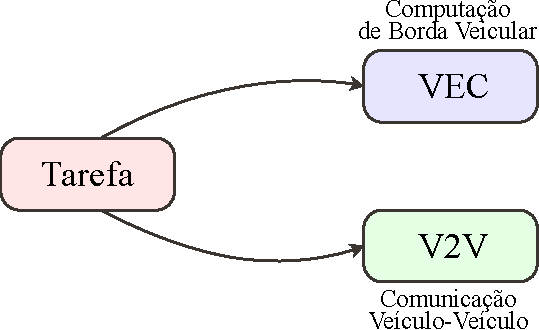
\includegraphics[width=0.9\textwidth]{figuras/task_vec_v2v.pdf}
        \end{column}
    \end{columns}
\end{frame}

% --- Slide 2.3: Alta mobilidade veicular ---
\begin{frame}{Mobilidade Veicular}
    \begin{columns}[T]
        \begin{column}{0.55\textwidth}
            \vspace{0.5cm}
            \begin{itemize}
                \item \textbf{Mudanças} constantes na \textbf{densidade} da rede e na \textbf{topologia} criam ambientes \textbf{incertos} (\underline{não estacionários})~\cite{he2025, luo2024}.
                \item \textbf{Intermitência} de sinal e \textbf{ruídos} nas \textbf{medições} de recursos~\cite{uddin2025, miriyala2026dl_offload_review}.
                \item Informações de \textbf{estado} podem \textbf{mudar rapidamente}.
            \end{itemize}
        \end{column}
        \begin{column}{0.5\textwidth}
            \centering
            \vspace{0.5cm}
            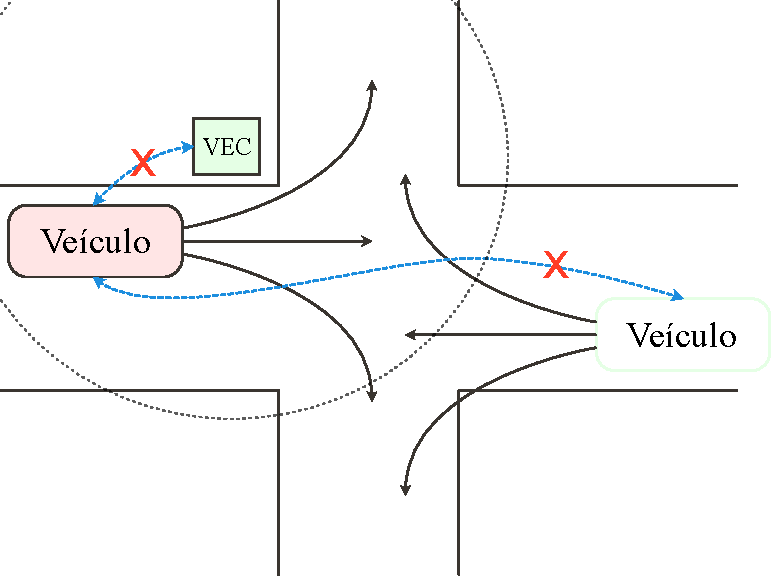
\includegraphics[width=0.9\textwidth]{figuras/mobilidade.pdf}
        \end{column}
    \end{columns}
\end{frame}

% --- Slide 2.4: Heurísticas determinísticas ---
\begin{frame}{Heurísticas}
    \begin{columns}[T]
        \begin{column}{0.5\textwidth}
            \begin{itemize}
                \item Heurísticas determinísticas \textbf{falham na adaptação} de longo prazo~\cite{cao2024survey, uddin2025}.
                \item Baseiam-se em conhecimento pontual (\textbf{\textit{snapshot}})~\cite{li2020genetic, you2021efficient}.
                \item Ignoram o impacto de ações sequenciais.
                \begin{itemize}
                    \item \textbf{Consumo} rápido de recursos.
                \end{itemize}
            \end{itemize}
        \end{column}
        \begin{column}{0.5\textwidth}
            \centering
            \vspace{0.5cm}
            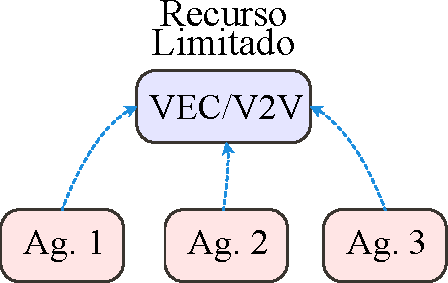
\includegraphics[width=0.7\textwidth]{figuras/heuristica.pdf}
        \end{column}
    \end{columns}
\end{frame}

% --- Slide 2.5: Modelos tradicionais de IA ---
\begin{frame}{\textit{Deep Reinforcement Learning} (DRL)}
    \begin{columns}[T]
        \begin{column}{0.55\textwidth}
            \vspace{0.5cm}
            \begin{itemize}
                \item Aprende no \textbf{longo prazo}.
                \item No entanto, exige \textbf{entrada} de dimensão \textbf{fixa}~ \cite{miriyala2026dl_offload_review, uddin2025}.
                \item Variações na topologia forçam \textbf{retreinamentos} onerosos.
            \end{itemize}
        \end{column}
        \begin{column}{0.45\textwidth}
            \centering
            \vspace{0.5cm}
            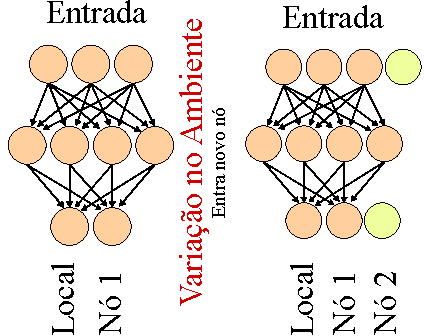
\includegraphics[width=0.9\textwidth]{figuras/drl.pdf}        \end{column}
    \end{columns}
\end{frame}

\begin{frame}{Revisão de Literatura}
    \large{Características do Ambiente Simulado}
    \begin{table}
        \centering
        \renewcommand{\arraystretch}{0.7}
        \resizebox{\textwidth}{!}{%
        \begin{tabular}{|l|c|c|c|c|c|c|c|c|}
            \hline
            \multirow{2}{*}{\textbf{Referência}} & \multirow{2}{*}{\textbf{5G}} & \multicolumn{2}{c|}{\textbf{Modo}} & \multirow{2}{*}{\textbf{VEC}} & \multirow{2}{*}{\textbf{ns-3}} & \multirow{2}{*}{\shortstack{\textbf{Mobilidade}\\\textbf{Real}}} & \multirow{2}{*}{\shortstack{\textbf{Incerteza}}} & \multirow{2}{*}{\shortstack{\textbf{Carga de Trabalho}\\\textbf{Real}}} \\ \cline{3-4}
                                             &   & \textbf{V2I}        & \textbf{V2V}              &   &   &            &   &            \\[1.5ex] \hline
            ~\cite{Moghaddasi2023}           & \checkmark   & \checkmark & -                & \checkmark & -   & -          & - & -          \\ \hline
            ~\cite{sidwini}                  & -            & \checkmark & -                & -          & -   & -          & - & -          \\ \hline
            ~\cite{li2025}                   & -            & \checkmark & -                & -          & -   & -          & - & \checkmark \\ \hline
            ~\cite{meghamala2025}            & \checkmark   & \checkmark & -                & -          & -   & -          & - & -          \\ \hline
            ~\cite{zhao2025}                 & -            & \checkmark & -                & \checkmark & -   & -          & - & -          \\ \hline
            ~\cite{mohammad2025}             & -            & \checkmark & \checkmark       & -          & -   & -          & - & -          \\ \hline
            ~\cite{xie2025}                  & -            & \checkmark & -                & \checkmark & -   & -          & - & -          \\ \hline
            ~\cite{wu2025ava}                & -            & \checkmark & \checkmark       & \checkmark & -   & -          & - & -          \\ \hline
            \textbf{TOLB}~\cite{wu2024}      & -            & \checkmark & -                & -          & -   & -          & - & -          \\ \hline
           \textbf{SAC-FTOPSIS} & \textbf{\checkmark} & \textbf{\checkmark} & \textbf{\checkmark} & \textbf{\checkmark} & \textbf{\checkmark} & \textbf{\checkmark} & \textbf{\checkmark} & \textbf{\checkmark} \\ \hline
        \end{tabular}%
        }
    \end{table}
\end{frame}

\begin{frame}{Revisão de Literatura}
    \large{Formulação}
    \begin{table}
        \centering
        \renewcommand{\arraystretch}{0.7}
        \resizebox{\textwidth}{!}{%
        \begin{tabular}{|l|c|c|c|c|c|}
            \hline
            \multirow{2}{*}{\textbf{Ref.}} & \multirow{2}{*}{\textbf{Alg.}} & \multirow{2}{*}{\shortstack{\textbf{Estado}\\\textbf{Invariante}}} & \multicolumn{2}{c|}{\textbf{Recompensa}} & \multirow{2}{*}{\shortstack{\textbf{Ação}\\\textbf{Binária}}} \\ \cline{4-5}
            & & & \textbf{GAP} & \shortstack{\textbf{Alinhada a}\\\textbf{Função Objetivo}} & \\ \hline
            ~\cite{Moghaddasi2023}          & DDQN   & -          & -          & -          & -          \\ \hline
            ~\cite{sidwini}                 & SAC    & -          & -          & -          & -          \\ \hline
            ~\cite{li2025}                  & DQN    & -          & -          & \checkmark & -          \\ \hline
            ~\cite{meghamala2025}           & SAC    & -          & -          & -          & -          \\ \hline
            ~\cite{zhao2025}                & DQN    & -          & -          & -          & -          \\ \hline
            ~\cite{mohammad2025}            & DDPG   & -          & -          & -          & -          \\ \hline
            ~\cite{xie2025}                 & PPO    & -          & -          & -          & -          \\ \hline
            ~\cite{wu2025ava}               & MADDPG & -          & -          & -          & -          \\ \hline
            \textbf{TOLB}~\cite{wu2024}     & TD3    & -          & -          & \checkmark & -          \\ \hline
            \textbf{SAC-FTOPSIS}            & \textbf{SAC} & \textbf{\checkmark} & \textbf{\checkmark} & \textbf{\checkmark} & \textbf{\checkmark} \\ \hline
        \end{tabular}%
        }
    \end{table}
\end{frame}

% --- Slide 7: Proposta ---
\section{Proposta}
\begin{frame}
    \centering
    \Huge \textbf{Proposta}
\end{frame}

% --- Slide 7.1: Questão de Pesquisa ---
\begin{frame}{Questão de Pesquisa}
    \vspace{1.5cm}
    \begin{center}
        \Large \textit{``Como tomar decisões de descarregamento de tarefas, utilizando DRL, em redes
VEC/V2X, com número variável de candidatos ao processamento, não-estacionariedade, de forma confiável e adaptativa, cumprindo restrições de prazo e minimizando latência e consumo energético, sem necessidade de retreinamento diante de variações na densidade veicular?''}
    \end{center}
\end{frame}

% --- Slide 7.2: Ideia central ---
\begin{frame}{Ideia central}
    \begin{itemize}
        \item Permitir que o \textbf{DRL} foque em otimizar a política de descarregamento de \textbf{longo prazo}.
        \item \textbf{Ranqueamento multicritério} dos nós candidatos~\cite{hwang1981}.
        \begin{itemize}
            \item Tornar o estado e as ações invariantes à escala.
        \end{itemize}
    \end{itemize}
\end{frame}

% --- Slide 7.3: SAC-FTOPSIS ---
\begin{frame}{SAC-FTOPSIS}
    \begin{columns}[T]
        \begin{column}{0.55\textwidth}
            \vspace{1cm}
            \begin{itemize}
                \item Divide a responsabilidade da decisão de descarregamento.
                \begin{itemize}
                    \item Agente DRL: decide ``\textbf{Quando}'' descarregar.
                    \item Módulo de ranqueamento: decide ``\textbf{Para onde}'' descarregar.
                \end{itemize}
            \end{itemize}
        \end{column}
        \begin{column}{0.45\textwidth}
            \centering
            \vspace{0.5cm}
            \begin{tikzpicture}[>=stealth, font=\sffamily]
                \node[block, fill=blue!10, minimum height=1.5cm] (when) {\textbf{DRL} \\ \scriptsize Quando?};
                \node[block, fill=orange!10, minimum height=1.5cm, below=1cm of when] (where) {\textbf{Ranqueamento} \\ \scriptsize Para onde?};
                
                \draw[arrow] (when) -- (where);
            \end{tikzpicture}
        \end{column}
    \end{columns}
\end{frame}

% --- Slide 7.4: Ranqueamento ---
\begin{frame}{Módulo de Ranqueamento}
    \begin{columns}[T]
        \begin{column}{0.55\textwidth}
            \vspace{0.5cm}
            \begin{itemize}
                \item O módulo de ranqueamento avalia a \textbf{qualidade} dos nós candidatos por \textbf{múltiplos critérios}.
                \begin{itemize}
                    \item Exemplo:
                    \begin{itemize}
                        \item Tempo de conclusão estimado (JCT).
                        \item Custo energético.
                        \item Distância até o nó candidato.
                    \end{itemize}
                \end{itemize}
                \item Identifica isoladamente a melhor alternativa de descarregamento (\textit{rank} 1).
            \end{itemize}
        \end{column}
        \begin{column}{0.45\textwidth}
            \centering
            \vspace{0.5cm}
            \begin{tikzpicture}[>=stealth, font=\sffamily]
                \node[rectangle, draw, fill=gray!10] (c1) at (0, 1) {JCT};
                \node[rectangle, draw, fill=gray!10] (c2) at (0, 0) {Energia};
                \node[rectangle, draw, fill=gray!10] (c3) at (0, -1) {Distância};
                
                \node[block, fill=orange!10] (eval) at (2.5, 0) {Ranquear};
                \node[circle, draw, fill=green!10] (r1) at (5, 0) {\textbf{\textit{Rank} 1}};
                
                \draw[arrow] (c1) -- (eval);
                \draw[arrow] (c2) -- (eval);
                \draw[arrow] (c3) -- (eval);
                \draw[arrow, thick] (eval) -- (r1);
            \end{tikzpicture}
        \end{column}
    \end{columns}
\end{frame}

% --- Slide 7.5: SAC ---
\begin{frame}{Agente DRL - SAC (\textit{Soft Actor-Critic})}
    \begin{itemize}
        \item Algoritmo \textbf{estado da arte}.
        \item \textbf{Equilibra} exploração e explotação otimizando simultaneamente a \textbf{recompensa} e a \textbf{entropia} da política~\cite{haarnoja2018sac}.
        \item Atributos arquiteturais e metodológicos:
        \begin{itemize}
            \item \textbf{\textit{Model-free}}, aprendendo diretamente a partir da interação com o ambiente.
            \item \textbf{\textit{Off-policy}}, garantindo alta eficiência amostral ao reavaliar decisões passadas.
            \item Utilização de \textbf{\textit{Replay Buffer}} para reaproveitar experiências e estabilizar o treinamento.
        \end{itemize}
    \end{itemize}
\end{frame}

% --- Slide 7.6: Estado invariante ---
\begin{frame}{Estado}
    \vspace{-0.2cm}
    \begin{equation*}
        s_t = \big[ \Delta_{obj}, \ U_{\text{local}}, \ U_{\text{rank 1}}, \ Q_{\text{local}}, \ Q_{\text{rank 1}}, \ C \big]
    \end{equation*}
    \begin{itemize}
        \item Vetor fixo de 6 dimensões:
        \begin{itemize}
            \item Ganho de tempo estimado ao descarregar ($\Delta_{obj}$).
            \item Urgência ($U_{\text{local}}$).
            \item Urgência ($U_{\text{rank 1}}$).
            \item Ocupação da fila de processamento ($Q_{\text{local}}$).
            \item Ocupação da fila de processamento ($Q_{\text{rank 1}}$).
            \item Complexidade da tarefa ($C$).
       \end{itemize}
        \item Captura a \textbf{urgência}, \textbf{ocupação da fila} e \textbf{complexidade} da tarefa independentemente do total de veículos.
    \end{itemize}
\end{frame}

% --- Slide 7.7: Ação e Recompensa ---
\begin{frame}{Ação e Recompensa}
    \begin{columns}[T]
        \begin{column}{0.45\textwidth}
            \vspace{0.2cm}
            \begin{itemize}
                \item Ação binária:
                \begin{itemize}
                    \item Processar \textbf{localmente}.
                    \item \textbf{Descarregar} para o melhor nó candidato (\textit{rank} 1).
                \end{itemize}
                \item Recompensa:
                \begin{itemize}
                    \item Divisão estrutural (GAP) entre \textbf{sucesso} e \textbf{falha}.
                    \item Ajuda a prevenir que o agente aprenda a falhar algumas vezes para economizar energia~\cite{ng1999policy}.
                \end{itemize}
            \end{itemize}
        \end{column}
        \begin{column}{0.55\textwidth}
            \centering
            \vspace{1cm}
            \begin{tikzpicture}[>=stealth, scale=0.9, transform shape, font=\sffamily]
                \draw[->, thick] (-3,0) -- (3,0);
                \draw[ultra thick, red] (-2.5,0.2) -- (-1,0.2) node[midway, above] {Falha};
                \draw[ultra thick, green!70!black] (0.5,0.2) -- (2.5,0.2) node[midway, above] {Sucesso};
                \draw[<->, dashed, thick] (-1,-0.3) -- (0.5,-0.3) node[midway, below] {GAP};
            \end{tikzpicture}
        \end{column}
    \end{columns}
\end{frame}

% --- Slide 8: Resultados preliminares ---
\section{Resultados Preliminares}
\begin{frame}
    \centering
    \Huge \textbf{Resultados preliminares}
\end{frame}

% --- Slide 8.1: Simulação ---
\begin{frame}{Simulação}
    \begin{itemize}
        \item Ambiente veicular (\textbf{cruzamento}):
        \begin{itemize}
            \item 1 VEC, 300m de alcance.
        \end{itemize}
        \item Mobilidade utilizando \textbf{SUMO}.
        \begin{itemize}
            \item Número variável de veículos.
        \end{itemize}
        \item Limitação térmica do processador (\textbf{\textit{throttling}}).
        \item Comunicação sujeita a \textbf{falhas}.
        \item Divulgação \textbf{atrasada} de capacidades dos nós candidatos.
        \item Carga real (\textbf{\textit{Alibaba Cluster}}).
        \item Modelo \underline{treinado} em cenário com \textbf{10} tarefas por segundo~(ts).
        \begin{itemize}
            \item \underline{Testado} com 10, 15, 20, 25, 30 e 45~ts.
        \end{itemize}
    \end{itemize}
\end{frame}

% --- Slide 8.2: Métricas ---
\begin{frame}{Métricas}
    \begin{itemize}
        \item \textbf{\% Sucesso}: Tarefa processada antes do prazo.
        \item \textbf{\% Local}: Porcentagem de tarefas processadas localmente.
        \item \textbf{SWQ (\textit{Success Weight Quality})}: Pondera taxa de sucesso e folga temporal.
        \item \textbf{$J(\pi)$ (Retorno Esperado)}: Recompensa acumulada pelo agente.
        \item \textbf{JCT (\textit{Job Completion Time})}: Tempo total (fila + rede + CPU).
        \item \textbf{Energia Consumida}: Gasto com processamento e transmissão.
    \end{itemize}
\end{frame}

% --- Slide 8.3: Resultados ---
\begin{frame}{Resultados Gerais}
    \centering
    \vspace{-0.2cm}
    \resizebox{0.95\textwidth}{!}{%
    \begin{tabular}{llrrrrrr}
    \toprule
    \textbf{Política} & \textbf{Categoria} & \textbf{\% Sucesso} & \textbf{SWQ} & \textbf{JCT (s)} & \textbf{E (J)} & \textbf{$J(\pi)$} & \textbf{\% Local} \\
    \midrule
    \multicolumn{8}{c}{\textbf{Proposta}} \\
    \midrule
    \rowcolor{green!10}\textbf{SAC-TOPSIS} $\star$ & \textbf{Proposta}   & \textbf{45,21} & \textbf{0,1484} & \textbf{6,547} & \textbf{25,828} & \textbf{0,2454} & \textbf{74,1} \\
    \midrule
    \multicolumn{8}{c}{\textbf{Heurísticas}} \\
    \midrule
    \textit{Greedy-Unfair} (Oráculo)      & Heurística          & 41,29 & 0,1262 & 5,613 & 7,396 & 0,2370 & 67,3 \\
    \textit{Random}                       & Heurística          & 30,02 & 0,0950 & 17,853 & 27,330 & 0,1427 & 40,7 \\
    VEC Pref.                    & Heurística          & 1,86  & 0,0030 & 144,191 & 4,843 & $-$0,1230 & 1,2 \\
    \midrule
    \multicolumn{8}{c}{\textbf{DRL Puro}} \\
    \midrule
    TD3-Base                     & DRL Puro            & 42,32 & 0,1418 & 6,045 & 24,414 & 0,2295 & 100,0 \\
    A2C-Base                     & DRL Puro            & 21,74 & 0,0772 & 13,653 & 48,862 & 0,0785 & 20,3 \\
    SAC-Base                     & DRL Puro            & 4,52  & 0,0119 & 57,075 & 24,230 & $-$0,0420 & 5,1 \\
    \midrule
    \multicolumn{8}{c}{\textbf{DRL+TOPSIS}} \\
    \midrule
    A2C-TOPSIS                   & DRL+TOPSIS          & 42,32 & 0,1418 & 6,045 & 24,414 & 0,2295 & 100,0 \\
    TD3-TOPSIS                   & DRL+TOPSIS          & 43,91 & 0,1388 & 3,703 & 22,995 & 0,2424 & 76,5 \\
    \bottomrule
    \end{tabular}%
    }
    
    \vspace{0.2cm}
    \raggedright
    \scriptsize \textit{*Nota: Os resultados são valores médios obtidos a partir de 658 cenários diferentes.}
\end{frame}

% --- Slide 9: Considerações Finais ---
\section{Considerações}
\begin{frame}
    \centering
    \Huge \textbf{Considerações}
\end{frame}

% --- Slide 9.1: Conclusão ---
\subsection{Contribuições Alcançadas}
\begin{frame}{Contribuições Alcançadas}
    \begin{itemize}
        \item O modelo híbrido conseguiu obter o melhor resultado em relação às outras políticas
        nos quesitos \textbf{taxa de sucesso}, \textbf{$J(\pi)$} e \textbf{SWQ}.
        \item \textbf{\textit{Greedy-Unfair}} consegue ser \underline{``melhor''} em algumas métricas pois conhece o \textbf{estado real} dos nós candidatos em cada \textbf{decisão}.  
        \begin{itemize}
            \item Apesar dessa imensa vantagem, \underline{\textbf{perde em \% Sucesso e SWQ}}.
        \end{itemize}
        \item \textbf{SWQ} ajuda a qualificar a taxa de sucesso.
        \item O uso do método de ranqueamento contribuiu para melhorar o $J(\pi)$ dos outros algoritmos DRL.
        \begin{itemize}
            \item A2C-Base (de 0,0785 para 0,2295).
            \item TD3-Base (de 0,2295 para 0,2424).
            \item SAC-Base (de $-$0,042 para 0,2454).
        \end{itemize}
    \end{itemize}
\end{frame}

% --- Slide 9.2: Trabalhos futuros ---
\subsection{Proposta Final}
\begin{frame}{Proposta Final}
    \begin{itemize}
        \item Incorporar \textbf{\textit{Fuzzy}-TOPSIS}.
        \item Integração ao \textbf{ns-3}.
        \item Cenários mais \textbf{desafiadores}.
    \end{itemize}
\end{frame}

% --- Slide 9.3: Cronograma ---
\subsection{Cronograma}
\begin{frame}{Cronograma de Pesquisa (2026--2028)}
    \centering
    \scriptsize
    \renewcommand{\arraystretch}{1.2}
    \begin{tabular}{|l|c|c|c|c|c|} 
        \hline
        \textbf{Atividade / Ano} & \multicolumn{2}{c|}{\textbf{2026}} & \multicolumn{2}{c|}{\textbf{2027}} & \textbf{2028} \\ \cline{2-6}
        & S1 & S2 & S1 & S2 & Q1 \\ \hline
        1. Exame de Qualificação            & \cellcolor{blue!15}X &   &   &   &   \\ \hline
        2. Integração com Simulador (ns-3/SUMO) & \cellcolor{blue!15}X & \cellcolor{blue!15}X &   &   &   \\ \hline
        3. Refinamento de Algoritmos        & \cellcolor{blue!15}X & \cellcolor{blue!15}X & \cellcolor{blue!15}X &   &   \\ \hline
        4. Avaliação de Desempenho          &   & \cellcolor{blue!15}X & \cellcolor{blue!15}X &   &   \\ \hline
        5. Análise dos Resultados           &   &   & \cellcolor{blue!15}X & \cellcolor{blue!15}X &   \\ \hline
        6. Escrita da Tese Final            &   &   &   & \cellcolor{blue!15}X & \cellcolor{blue!15}X \\ \hline
        7. Defesa Final                     &   &   &   &   & \cellcolor{blue!15}X \\ \hline
    \end{tabular} 
    
    \vspace{0.4cm}
    \tiny \textbf{Legenda}: S1: 1º semestre; S2: 2º semestre; Q1: 1º trimestre de 2028.
\end{frame}

\section{Referências}
%%################ Referências #############
\begin{frame}[allowframebreaks]{Referências}
\bibliographystyle{ieeetr}
\bibliography{biblio}
\end{frame}


\begin{frame}
    \maketitle
\end{frame}

\end{document}
